% Construction : f(x) = x[2(ln x)² − 3 ln x + 2], et sa tangente y = 2x − e au
% point B(e ; e). Le domaine hachuré est compris entre la courbe et la tangente,
% de x = 1 à x = e ; son aire vaut (3e² − 4e − 5)/4.
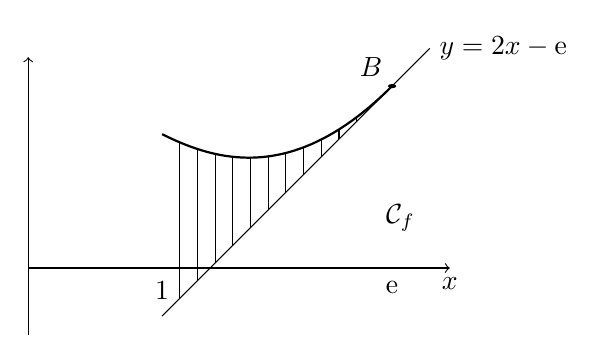
\begin{tikzpicture}[xscale=1.7, yscale=0.85]
  \draw[->] (0, 0) -- (3.15, 0) node[below] {$x$};
  \draw[->] (0, -1) -- (0, 3.15);
  \draw[thin] (1.1322, -0.4539) -- (1.1322, 1.8776);
  \draw[thin] (1.2644, -0.1896) -- (1.2644, 1.7781);
  \draw[thin] (1.3965, 0.0748) -- (1.3965, 1.7053);
  \draw[thin] (1.5287, 0.3391) -- (1.5287, 1.6617);
  \draw[thin] (1.6609, 0.6035) -- (1.6609, 1.6489);
  \draw[thin] (1.7931, 0.8678) -- (1.7931, 1.6678);
  \draw[thin] (1.9252, 1.1322) -- (1.9252, 1.7193);
  \draw[thin] (2.0574, 1.3965) -- (2.0574, 1.8036);
  \draw[thin] (2.1896, 1.6609) -- (2.1896, 1.9209);
  \draw[thin] (2.3218, 1.9252) -- (2.3218, 2.0711);
  \draw[thin] (2.4539, 2.1896) -- (2.4539, 2.2542);
  \draw[thin] (2.5861, 2.4539) -- (2.5861, 2.4700);
  \draw[thick] plot coordinates {(1.0000, 2.0000) (1.0430, 1.9580) (1.0859, 1.9181) (1.1289, 1.8804) (1.1718, 1.8451) (1.2148, 1.8125) (1.2577, 1.7825) (1.3007, 1.7553) (1.3437, 1.7311) (1.3866, 1.7098) (1.4296, 1.6916) (1.4725, 1.6766) (1.5155, 1.6647) (1.5584, 1.6561) (1.6014, 1.6508) (1.6444, 1.6487) (1.6873, 1.6501) (1.7303, 1.6548) (1.7732, 1.6629) (1.8162, 1.6745) (1.8591, 1.6895) (1.9021, 1.7079) (1.9451, 1.7298) (1.9880, 1.7552) (2.0310, 1.7841) (2.0739, 1.8164) (2.1169, 1.8523) (2.1598, 1.8916) (2.2028, 1.9344) (2.2458, 1.9807) (2.2887, 2.0305) (2.3317, 2.0837) (2.3746, 2.1404) (2.4176, 2.2006) (2.4605, 2.2643) (2.5035, 2.3314) (2.5465, 2.4019) (2.5894, 2.4759) (2.6324, 2.5533) (2.6753, 2.6341) (2.7183, 2.7183)};
  \draw (1, {2 - 2.71828}) -- (3, {6 - 2.71828});
  \fill (2.71828, 2.71828) circle (0.9pt);
  \node[above left] at (2.71828, 2.71828) {$B$};
  \node[below] at (1, -0.06) {$1$};
  \node[below] at (2.71828, -0.06) {$\mathrm{e}$};
  \node[right] at (2.6, 0.75) {$\mathcal{C}_f$};
  \node[right] at (3, 3.28) {$y = 2x - \mathrm{e}$};
\end{tikzpicture}
